% Template created by Karol Kozioł (www.karol-koziol.net) for ShareLaTeX

\documentclass[a4paper,9pt]{extarticle}
\usepackage[utf8]{inputenc}
\usepackage[T1]{fontenc}
\usepackage{graphicx}
\usepackage[usenames,dvipsnames]{xcolor}
\usepackage{tikz}

\usepackage{amsmath,amssymb,textcomp}
\everymath{\displaystyle}

\usepackage{times}
\renewcommand\familydefault{\sfdefault}
\usepackage{tgheros}
% \usepackage[defaultmono,scale=0.85]{droidmono}

\usepackage{multicol}
\setlength{\columnseprule}{0pt}
\setlength{\columnsep}{20.0pt}
\usepackage{enumitem}
\usepackage{booktabs}
\usepackage{tabularx}
\usepackage{array}
\usepackage{mdframed}

\newcolumntype{L}[1]{>{\raggedright\let\newline\arraybackslash\hspace{0pt}}m{#1}}
\newcolumntype{C}[1]{>{\centering\let\newline\arraybackslash\hspace{0pt}}m{#1}}
\newcolumntype{R}[1]{>{\raggedleft\let\newline\arraybackslash\hspace{0pt}}m{#1}}


\usepackage{geometry}
\geometry{
a4paper,
total={210mm,297mm},
left=10mm,right=10mm,top=10mm,bottom=15mm}

\usepackage[acronym]{glossaries}
\usepackage{acronym}
\linespread{1.3}

\usepackage[colorlinks = true,
            linkcolor = blue,
            urlcolor  = blue,
            citecolor = blue,
            anchorcolor = blue]{hyperref}
% custom title
\makeatletter
\renewcommand*{\maketitle}{%
\noindent
\begin{minipage}{\textwidth}
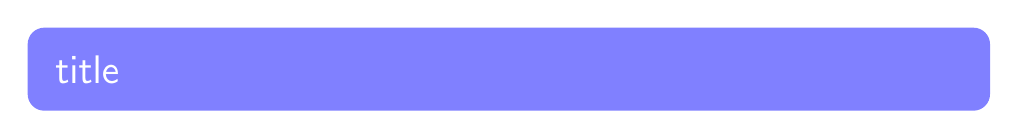
\begin{tikzpicture}
\node[rectangle,rounded corners=6pt,inner sep=10pt,fill=blue!50,text width= 0.95\textwidth] {
% \begin{tabular}{;r}
\color{white}\Large
% \end{tabular}
\@title};
\end{tikzpicture}
% \begin{tikzpicture}
% \node[rectangle,rounded corners=6pt,inner sep=10pt,fill=blue!50,text width= 0.95\textwidth] 
% {\color{white}\large \@subtitle};
% \end{tikzpicture}
\end{minipage}
% \hfill
% \begin{minipage}{0.55\textwidth}
% \begin{tikzpicture}
% \node[rectangle,rounded corners=3pt,inner sep=10pt,draw=blue!50!black,text width= 0.95\textwidth] { \@author};
% \end{tikzpicture}
% \end{minipage}
\bigskip\bigskip
}%
\makeatother

\newcommand{\com}[1]{\textcolor{red}{#1}}
\newcommand{\ie}{\textit{i}.\textit{e}., }
\newcommand{\eg}{\textit{e}.\textit{g}., }
\newcommand*{\etc}{etc.\@\xspace}

\newacronym{fiw}{FIW}{Families In the Wild}
\newacronym{lfw}{LFW}{Labeled Faces in the Wild}
\newacronym{fd}{FD}{Father-Daughter}
\newacronym{ms}{MS}{Mother-Son}

% % custom title
% \makeatletter
% \renewcommand*{\maketitle}{%
% \noindent
% \begin{minipage}{\textwidth}
% \begin{tikzpicture}
% \node[rectangle,rounded corners=6pt,inner sep=10pt,fill=blue!50,text width= 0.95\textwidth] {\color{white}\Huge \@title};
% \end{tikzpicture}
% \begin{tikzpicture}
% \node[rectangle,rounded corners=6pt,inner sep=10pt,fill=blue!50,text width= 0.95\textwidth] 
% {\color{white}\large \@subtitle};
% \end{tikzpicture}
% \end{minipage}
% \hfill
% \begin{minipage}{0.55\textwidth}
% \begin{tikzpicture}
% \node[rectangle,rounded corners=3pt,inner sep=10pt,draw=blue!50!black,text width= 0.95\textwidth] {\LARGE \@author};
% \end{tikzpicture}
% \end{minipage}
% \bigskip\bigskip
% }%
% \makeatother

% custom section
\usepackage[explicit]{titlesec}
\titleformat{\chapter}
  {\centering\Large\bfseries} % format
  {}% label
  {0pt} % sep
  {\huge}  
  
%   \titleformat{\section}{\normalfont\Large\centering\bfseries}{\thesection}{1em}{\uppercase\centering}


\newcommand*\sectionlabel{}
\titleformat{\section}
  {\gdef\sectionlabel{}
  \normalfont\sffamily\Large\bfseries\scshape}
  {\gdef\sectionlabel{\thesection\ }}{0pt}
  {
\noindent
\begin{tikzpicture}[scale=2]
\node[rectangle, text centered,rounded corners=3pt,ultra thick,fill=Blue!80,text width= 0.95\columnwidth] {\color{white}\sectionlabel#1};
% \node[rectangle,rounded corners=3pt,inner sep=4pt,fill=Peach!50,text width= 0.95\columnwidth] {\color{white}\sectionlabel#1};
\end{tikzpicture}
  }
 \usepackage[english]{babel}

\titlespacing*{\section}{0pt}{15pt}{10pt}
\newcounter{step}[section]
\newenvironment{step}[2][]
{% begin code 
    \refstepcounter{step}\par\medskip
    \noindent\textbf{Step~\thestep. #1}{\textbf{#2}:}\rmfamily
}%
{\medskip}
   

% custom footer
\usepackage{fancyhdr}
\makeatletter
\pagestyle{fancy}
\fancyhead{}
\fancyfoot[C]{\footnotesize \textcopyright\ \@date\ \ \@author}
\renewcommand{\headrulewidth}{0pt}
\renewcommand{\footrulewidth}{0pt}
\makeatother


\title{\color{white}\LargeA Database for Studying Visual Kinship Recognition Systems \hspace{48mm} FIW Database}

\author{Joseph Robinson, Northeastern University, MA}
% * <mzhang1.student@thehudsonschool.org> 2017-03-30T13:34:20.173Z:
%
% ^.
\date{August 2019}


%
\newcommand{\abs}[1]{\left| #1 \right|}
%\renewcommand{\vec}[1]{\mathbf{#1}}
%
\usepackage{blindtext}

\begin{document}

\maketitle
\begin{multicols}{2}


% \section*{Trigonometry}

\section*{Motivation}
\subsection*{Why was the dataset created?} 
% For instance, was there a specific task in mind? was there a specific gap that needed to be filled?
\noindent \gls{fiw} was created to provide images that can be used to study automatic kinship recognition in the unconstrained setting: settings vary across several characteristics (\eg pose, illumination, resolution, focus,), demographics (\eg age, gender, race), appearances (\eg hairstyle, makeup, clothing), and familial meta-data (\ie families of different sizes that consist of different relationship types). The dynamic nature of the labels allows for data to be parsed for various tasks and applications. Amongst the possible tasks, is the most popular kinship verification task based on face-pair matching: given a pair of facial images, determine whether or not the images are blood relatives.
\subsection*{Who created this dataset (\eg which team, research group) and on behalf of which entity (\eg company, institution, organization)?}
The initial version of \gls{fiw} was created by Joseph P. Robinson, Ming Shao, and Yun Fu, whom were researchers at the Northeastern University's SMILE Lab at the time of its initial release in 2017.
\subsection*{Who funded the creation of the dataset?}
% If there is an associated grant, please provide the name of the grantor and the grant name and number.
N/A



\section*{Composition}
\subsection*{What are the instances? (that is, examples; \eg documents, images, people, countries) Are there multiple types of instances? (\eg movies, users, ratings; people, interactions between them; nodes, edges)}
\noindent
{\color{red} The instances of the dataset are pictures of faces, with one face per image.} 

\subsection*{Are relationships between instances made explicit in the data (\eg social network links, user/movie ratings, etc.)?}
\noindent
{\color{red} Yes. The data is organized into a two-level hierarchy of folders, with each top-level folder in the hierarchy representing a family. In addition, a relationship adjacency matrix containing all members of the family as nodes is provided.} 

\subsection*{How many instances are there? (of each type, if appropriate)?}
\noindent

\subsection*{What data does each instance consist of? “Raw” data (\eg unprocessed text or images)? Features/attributes? Is there a label/target associated with instances? If the instances related to people, are subpopulations identified (\eg by age, gender, etc.) and what is their distribution?}
\noindent Each instance is a pair of subjects labeled with the name of the
person in the image. Some images contain more than one face.
The labeled face is the one containing the central pixel of the
image—other faces should be ignored as “background”.

\subsection*{Is everything included or does the data rely on external resources?
(\eg websites, tweets, datasets) If external resources, a) are there guarantees that they will exist, and remain constant, over time; b) is there an official archival version; c) are there access restrictions or fees?}
\noindent The dataset is self-contained.

\subsection*{Are there recommended data splits and evaluation measures? (\eg training, development, testing; accuracy or AUC)}
\noindent The dataset comes with specified train/test splits such that there is no family overlap between sets. Therefore, no subject overlap between folds either. The data organized as a table of pairs (datatable.csv or datatable.pkl). Each item is listed with following values across the columns: 'fid', 'fold', 'label', 'p1', 'p2', 'type'. 'fid' indicates the family ID as referenced in \gls{fiw}, 'fold' indicates the fold to hold the element out for testing (\ie with remaining folds making up the training set). 'p1' and 'p1' are sample face 1 and 2, respectfully (\ie facial pair). 'label; is ground-truth (\ie 0 if unrelated and 1 if related/ true pair). Finally, 'type indicates the relationship in question (\eg \gls{ms}, \gls{fd}, \etc).

Practitioners train algorithms on the training set and evaluate on the test set in a 5-fold fashion. Final
performance results are averaged across folds alongside the respective standard deviation.
In other words, there are 5 train/test subsets of the dataset-each fold, leave out its items for testing, train on other K-1 (\ie 5-1=4) folds, then evaluate on test set unseen \wrt model trained from other folds. This way, all data is used for testing. Furthermore, different training paradigms are allowed while mantaining frozen test sets. As such, we recommend reporting performance on all folds by using leave-one-out cross validation, performing 5 experiments. That is, in each experiment, 4 subsets should be used as a training set and the 5th subset should be used for testing. At a minimum, we recommend reporting the estimated mean accuracy, $$\hat\mu=\frac{\sum^K_{k=1}p_k}{K},$$ where K=5 and $p_k$ is percentage of correct classifications for fold $k$. Along with the standard error of the mean $S_E$ as
$$
\mu=\frac{\hat\sigma}{\sqrt{K}},
$$
where $\hat\sigma$ is the estimate of the standard deviation, defined as
$$
\mu=\sqrt{\frac{\sum^K_{k=1}(p_k-\hat\mu)^2}{K 1}}.$$

\paragraph{Training Paradigms:} As the renowned \gls{lfw}, \gls{fiw} supports three training paradigms for the verification task, with the first two the preferred of \gls{fiw} creators and organizers, however, we decided to include to avoid having reported results that fall outside the two preferred paradigms. Practitioners must clearly state the paradigm followed for all published results.

% \begin{itemize}
\begin{step}{List-Restricted for Training.}\label{1ststep} 
This setting does not allow for the family or subject names to be referenced during training or testing. The only labels provided are the ground-truth boolean tags: whether or not a pair of images consist of faces of relatives, and not the identity of the person or any knowledge about family name. Under this paradigm, determining whether multiple pairs of images in the train/test set that belong to the same person(s) and/or family(s) is non-trivial. Such inferences, however, might be made by performing conventional face verification across all pair-wise combinations (\ie opposed to comparing FID.MID references). Thus, training pairs made-up of matched and mismatched pairs, one can use image equivalence to cluster faces of the same family and even a finer-level of person ID. Pair-list file datatable\_restricted.csv is provided with only the labels allowed in this paradigm (\ie essentially the master-pairs-list file with only columns ['p1', 'p2', 'label']).
    \end{step}
    \begin{step}{List-Unrestricted for Training.} This setting allows referencing to the family, subjects, and particular type of relationship bonding the pairs of matched faces, while also providing this same information for the mismatched (\ie same number of negatives were generated for each type, however, currently types are just being used for analysis of the different types, though certainly possible to leverage knowledge of specific type during training. The file fidlist.csv lists all the family IDs (FIDs), number of members (\ie member IDs (MIDs)), along with the total number of faces (\ie face IDs (faceIDs)) between all mumbers of respective family. Matched and mismatched pairs should be used directly as provided in pair-lists. For instance, when processing fold-1, the FIDs of this fold and all pairs they make-up are held out for testing (\ie frozen as provided in list). For this, positive\_pairs.csv is provided with fields for 'p1', 'p2', and 'fold'. For instance, say training pair is F0001.MID1-F0001.MID3 are true kin of type \gls{fd}, if the former has 5 facial images and the latter has 3 it is then possible to create $$\binom{n}{2}=\binom{5+3}{2}=28$$. Hence, the practitioner can create arbitrary matching/mismatching pairs to best suit their system. Any pairings created and added to list, whether true or false matches, should only be done on training splits, as the unrestricted paradigm allows training list to be created, but not for performance to be reported. The test data of each fold should remain frozen (\ie unmodified listing of pairs), which then provides platform for fair comparison of performance ratings. We recommend that experimenters first use the List-Restricted paradigm (\ie use provided lists for both train and test). Then, evolve to the List-Unrestricted paradigm if it is believed that the prospective system would benefit from training with more pairs, more metadata, pairs spanning best representation, \etc. In other words, if it seems benefit could be had by modifying list of training items then move from List-Restricted (above) to List-Unrestricted (this). 
     \end{step}
    
    
\begin{step}{Unrestricted for Training.} Inherits all characterizations of List-Unrestricted paradigm, but now outside data is allowed to be added to the training. This paradigm is discouraged, as newer, larger versions of \gls{fiw} will be continually released and, hence, it will be made sure that no subjects added during training are in anyway a part of testing (\ie not even a subject related to member of test set). Nonetheless, if this paradigm is followed, extensive reporting on the process, sources, and amounts added during training.
 \end{step}
Regardless the case, \textbf{it should be made clear which of these two paradigms are followed.}
% \end{itemize}

\subsection*{What experiments were initially run on this dataset? Have a summary of those results.}
\noindent \textcolor{red}{
Four different types of experiments were initially performed on FIW. Those experiments were:  benchmarking kinship verification and family classification; evaluating the proposed semi-supervised clustering method; evaluating CNNs fine-tuned using FIW on KinWild I \& II (i.e., transfer-learning), and measuring human performance on kinship verification with a comparison to top-performing algorithms from previous experiments.} 
\subsubsection*{\textcolor{red}{Kinship Verification}}
\textcolor{red}{
SphereFace, which was fine-tuned on FIW, outperformed other benchmarks with an average accuracy of 69.18 percent, which is 1.31 and 2.11 percent better than ResNet-22+CF and mDML, respectively, which were top the scoring methods prior to the recent release of SphereFace. The highest verification accuracies were achieved on siblings pair types followed by parent-child types, and then grandparent-grandchild. Thus, the wider the generational gap, the wider between appearances of faces.
}

\subsubsection*{\textcolor{red}{Family Classification}}
\textcolor{red}{
The top performance was with the fine- tuned ResNet-22 using Centerface loss with 16.18\%. The naive baseline approach (one-vs-rest linear SVMs on top of deep VGG-Face features) achieved an accuracy of just 3.04 per- cent. Then, by replacing the softmax layer to target the num- ber of families (i.e., 564), and fine-tuning on FIW, the top-1 accuracy was improved (i.e., +7.38 to 10.42 percent)
}

\subsubsection*{\textcolor{red}{Semi-supervised Clustering}}
\textcolor{red}{
Even on the unlabeled data, the proposed method exceeds the K-means baseline. For LCVQE, the pair-wise constraints make the cluster structure unpredictable, vulnerable to deviate from the true one, and, thus, perform worse than the K-means baseline.
}

\subsubsection*{\textcolor{red}{Transfer Learning}}
\textcolor{red}{
The fine tuned network (ResNet + Centerface) performed better in average accuracy than all other methods, while providing less variation in type-specific scores. For KinWild I, we get a 4 percent increase in performance (i.e., from 78.4 to 82.4 percent). For KinWild II, there is a 5.6 percent improvement to 86.6 percent.
}

\subsubsection*{\textcolor{red}{Human Performance on FIW}}
\textcolor{red}{
Human judges had a mean accuracy of 57.5\% with significant variance in accuracy 
NEEDS TO BE FILLED IN
}



\subsection*{Any other comments?}

\subsection*{Is the dataset self-contained, or does it link to or otherwise rely on external resources (\eg websites, tweets, other datasets)?}
% If it links to or relies on external resources, a) are there guarantees that they will exist, and remain constant, over time; b) are there official archival versions of the complete dataset (\ie including the external resources as they existed at the time the dataset was created); c) are there any restrictions (\eg licenses, fees) associated with any of the external resources that might apply to a future user? Please provide descriptions of all external resources and any restrictions associated with them, as well as links or other access points, as appropriate.
\noindent The dataset is self-contained.

\subsection*{Does the dataset contain data that might be considered confidential (\eg data that is protected by legal privilege or by doctorpatient confidentiality, data that includes the content of individuals non-public communications)?}
% If so, please provide a description. 

\noindent No. All data was derived from publicly available news sources. 

\subsection*{Does the dataset contain data that, if viewed directly, might be offensive, insulting, threatening, or might otherwise cause anxiety?}
% \texttt{If so, please describe why.}}
No. The dataset only consists of faces and associated names.

\subsection*{Does the dataset relate to people?}
% \texttt{If not, you may skip the remaining questions in this section.}}\
\noindent Yes. The dataset contains one or more face images of individuals.


\subsection*{Does the dataset identify any subpopulations (\eg by age, gender)?}
% \texttt{If so, please describe how these subpopulations are identified and provide a description of their respective distributions within the dataset.}}

\noindent While sub-population data was not available at the initial release of the dataset, a subsequent paper2 reports the distribution of images by age, race and gender. Table 2 lists these results. The age, perceived gender and race of each individual in the dataset was collected using Amazon Mechanical Turk, with 3 crowd workers labeling each image. After exact age estimation, the ages were binned into groups of 0-10, 21-40, 41-60 and 60+. 

\subsection*{Is it possible to identify individuals (\ie one or more natural persons), either directly or indirectly (\ie in combination with other data) from the dataset?}
% If so, please describe how.
\noindent Each image is annotated with the name of the person that appears
in the image.

\subsection*{Does the dataset contain data that might be considered sensitive in any way (\eg data that reveals racial or ethnic origins, sexual orientations, religious beliefs, political opinions or union memberships, or locations; financial or health data; biometric or genetic data; forms of government identification, such as social security numbers; criminal history)?}
% \texttt{If so, please provide a description.}}
\noindent The dataset does not contain confidential information since all information was scraped from news stories. 

\subsection*{Any other comments?}

% \begin{center}

% \start{tabular}{P{2.5cm}} \end{tabular}
\section*{Data Collection Process}

% \end{center}
\subsection*{How was the data associated with each instance acquired? \texttt{Was the data directly observable (\eg raw text, movie ratings), reported by subjects ((\eg survey responses), or indirectly inferred/derived from other data (\eg part-of-speech tags, model-based guesses for age or language)? If data was reported by subjects or indirectly inferred/derived from other data, was the data validated/verified? If so, please describe how.}}

\noindent The names for each person in the dataset were determined by an
operator by looking at the caption associated with the person’s
photograph.

\subsection*{What mechanisms or procedures were used to collect the data (\eg hardware apparatus or sensor, manual human curation, software program, software API)?}
% How were these mechanisms or procedures validated?
\noindent The raw images for this dataset were obtained from the Faces in
the Wild database collected by Tamara Berg at Berkeley3. The images in this database were gathered from news articles on the web using software to crawl news articles.


\subsection*{If the dataset is a sample from a larger set, what was the sampling strategy (\eg deterministic, probabilistic with specific sampling probabilities)?}

\noindent The original Faces in the Wild dataset is a sample of pictures of people appearing in the news on the web. Labeled Faces in the
Wild is thus also a sample of images of people found on the news
on line. While the intention of the dataset is to have a wide range
of demographic (e.g. age, race, ethnicity) and image (e.g. pose,
illumination, lighting) characteristics, there are many groups that
have few instances (e.g. only 1.57\% of the dataset consists of
individuals under 20 years old).

\subsection*{Who was involved in the data collection process (\eg students, crowdworkers, contractors) and how were they compensated (\eg
how much were crowdworkers paid)?}

\noindent Students of NEU.

\subsection*{Over what timeframe was the data collected?}
% \texttt{Does this timeframe match the creation timeframe of the data associated with the instances (\eg recent crawl of old news articles)? If not, please describe the timeframe in which the data associated with the instances was created




\subsection*{Were any ethical review processes conducted (\eg by an institutional review board)?}
% If so, please provide a description of these review processes, including the outcomes, as well as a link or other access point to any supporting documentation.
\noindent Unknown


\subsection*{Does the dataset relate to people?}
% If not, you may skip the remaining questions in this section.
\noindent Yes. Each instance is an image of a person.

\subsection*{Did you collect the data from the individuals in question directly, or obtain it via third parties or other sources (\eg websites)?}
\noindent The data was crawled from public web sources.

\subsection*{Were the individuals in question notified about the data collection? \texttt{If so, please describe (or show with screenshots or other information) how notice was provided, and provide a link or other access point to, or otherwise reproduce, the exact language of the notification itself.}}
\noindent Unknown

\subsection*{Did the individuals in question consent to the collection and use of their data?}
%If so, please describe (or show with screenshots or other information) how consent was requested and provided, and provide a link or other access point to, or otherwise reproduce, the exact language to which the individuals consented.

\noindent No. All subjects in the dataset appeared in news sources so the
images that we used along with the captions are already public.

\subsection*{If consent was obtained, were the consenting individuals provided with a mechanism to revoke their consent in the future or for certain uses?}
% If so, please provide a description, as well as a link or other access point to the mechanism (if appropriate).
\noindent No. The data was crawled from public web sources, and the individuals appeared in news stories. But there was no explicit informing of these individuals that their images were being assembled into a dataset.

\subsection*{Has an analysis of the potential impact of the dataset and its use on data subjects (\eg a data protection impact analysis)been conducted?}
%  If so, please provide a description of this analysis, including the outcomes, as well as a link or other access point to any supporting documentation.
\noindent Unknown

\subsection*{Any other comments?}
\noindent 

\subsection*{\texttt{d}}
\noindent 

\subsection*{How was the data collected? (\eg hardware apparatus/sensor, manual human curation, software program, software interface/API)}
\noindent


\subsection*{Who was involved in the data collection process? (\eg students, crowdworkers) and how were they compensated (\eg how much were crowdworkers paid)?}
\noindent Several student volunteers, along with experts overseeing many of the details. No monetary cost was acquired for this effort.

\subsection*{Over what time-frame was the data collected? Does the collection timeframe match the creation time-frame of the instances?}
\noindent
\textcolor{red}{
The dataset was created over a timescale of months. The collection timeframe does not match the creation timeframe.}


\subsection*{Does the dataset contain all possible instances? Or is it a sample (not necessarily random) of instances from a larger set?}
\noindent
\subsection*{If the dataset is a sample, then what is the population? What was the sampling strategy (\eg deterministic, probabilistic with specific sampling probabilities)? Is the sample representative of the larger set (\eg geographic coverage)? If not, why not (\eg to cover a more diverse range of instances)? How does this affect possible uses?}
\noindent
\subsection*{Is there information missing from the dataset and why? (this does not include intentionally dropped instances; it might include, \eg redacted text, withheld documents) Is this data missing because it was unavailable?}
\noindent
\textcolor{red}{
No information is missing.
}

\section*{Data Preprocessing}
\subsection*{What preprocessing/cleaning was done? (\eg discretization or bucketing, tokenization, part-of-speech tagging, SIFT feature extraction, removal of instancess, processing of missing values)?}
% \texttt{If so, please provide a description. If not, you may skip the remainder of the questions in this section.}}
\noindent The following steps were taken to process the data:
\begin{enumerate}

\item \paragraph{Gathering raw images} First the raw images for this
dataset were obtained from the Faces in the Wild dataset
consisting of images and associated captions gathered from
news articles found on the web.
2. Running the Viola-Jones face detector4 The OpenCV version 1.0.0 release 1 implementation of Viola-Jones face detector was used to detect faces in each of these images, using
the function cvHaarDetectObjects, with the provided Haar
classifier—cascadehaarcascadefrontalfacedefault.xml. The
scale factor was set to 1.2, min neighbors was set to 2, and
the flag was set to CV HAAR DO CANNY PRUNING.
3. Manually eliminating false positives: If a face was detected and the specified region was determined not to be a
face (by the operator), or the name of the person with the
detected face could not be identified (using step 5 below),
the face was omitted from the dataset.
4. Eliminating duplicate images: If images were determined
to have a common original source photograph, they are defined to be duplicates of each other. An attempt was made to
remove all duplicates but a very small number (that were not
initially found) might still exist in the dataset. The number
of remaining duplicates should be small enough so as not
to significantly impact training/testing. The dataset contains
distinct images that are not defined to be duplicates but are
extremely similar. For example, there are pictures of celebrities that appear to be taken almost at the same time by different photographers from slightly different angles. These
images were not removed.
5. Labeling (naming) the detected people: The name associated with each person was extracted from the associated
\end{enumerate}

\subsection*{Was the “raw” data saved in addition to the preprocessed/cleaned data? (\eg to support unanticipated future uses)}
\noindent
\subsection*{Is the preprocessing software available?}
\noindent
\subsection*{Does this dataset collection/processing procedure achieve the motivation for creating the dataset stated in the first section of this datasheet? If not, what are the limitations?}
\noindent

\section*{Dataset Distribution}
\subsection*{How will the dataset be distributed? (\eg tarball on website, API, GitHub; does the data have a DOI and is it archived redundantly?)}
\noindent
\subsection*{When will the dataset be released/first distributed?}
\noindent
\subsection*{What license (if any) is it distributed under? Are there any copyrights on the data?}
\noindent
\subsection*{Are there any fees or access/export restrictions?}
\noindent


\section*{Dataset Maintenance}
\subsection*{Who is supporting/hosting/maintaining the dataset?}
\noindent
\subsection*{Will the dataset be updated? If so, how often and by whom? Unknown
How will updates be communicated? (\eg mailing list, GitHub)}
\noindent
\subsection*{Is there an erratum?}
\noindent
\subsection*{If the dataset becomes obsolete how will this be communicated?}
\noindent
\subsection*{Is there a repository to link to any/all papers/systems that use this dataset?}
\noindent
\subsection*{If others want to extend/augment/build on this dataset, is there a mechanism for them to do so? If so, is there a process for tracking/assessing the quality of those contributions. What is the process for communicating/distributing these contributions to users?}
\noindent

\section*{Uses}
\subsection*{What (other) tasks could the dataset be used for?}
\noindent Family classification, large scale search \& retrieval, fine-grained categorization, tri-subject verification, hierarchical clustering, to name a few.


\subsection*{Has the dataset been used for any tasks already? \texttt{If so, where are the results so others can compare (\eg links to published papers)?}}
\noindent 
\subsection*{Has the dataset been used for any tasks already? \texttt{If so, please provide a description.}}
Papers using this dataset and the specified evaluation protocol are
listed in http://vis-www.cs.umass.edu/lfw/results.html
\subsection*{Is there a repository that links to any or all papers or systems that use the dataset? \texttt{If so, please provide a link or other access point.}}
Papers using this dataset and the specified training/evaluation
protocols are listed under “Methods” section of http://vis-www.cs.
umass.edu/lfw/results.html
\subsection*{What (other) tasks could the dataset be used for?}
The LFW dataset can be used for the face identification problem.
Some researchers have developed protocols to use the images in
the LFW dataset for face identification.5
\subsection*{Is there anything about the composition of the dataset or the way it was collected and preprocessed/cleaned/labeled that might impact
future uses? \texttt{For example, is there anything that a future user might need to know to avoid uses that could result in unfair treatment of individuals or groups (\eg stereotyping, quality of service issues) or other undesirable harms (\eg financial harms, legal risks) If so, please provide a description. Is there anything a future user could do to mitigate these undesirable harms?}}

There is minimal risk for harm: the data was already public.
\subsection*{Are there tasks for which the dataset should not be used?}
% \texttt{If so, please provide a description.The dataset should not be used for tasks that are high stakes (e.g. law enforcement).}
\subsection*{Any other comments?}


\end{multicols}



\section*{Elementary Power Series}


\begin{align*}
CMC
\end{align*}



\newpage

\begin{multicols}{2}

\newpage

%\section*{Trigonometry}


\section*{Legal \& Ethical Considerations}
\subsection*{If the dataset relates to people (\eg their attributes) or was generated by people, were they informed about the data collection? (\eg datasets that collect writing, photos, interactions, transactions, etc.)}
\noindent


\subsection*{If it relates to people, were they told what the dataset would be used for and did they consent? If so, how? Were they provided with any mechanism to revoke their consent in the future or for certain uses?}
\noindent

\subsection*{If it relates to people, could this dataset expose people to harm or legal action? (\eg financial social or otherwise) What was done to mitigate or reduce the potential for harm?}
\noindent

\subsection*{If it relates to people, does it unfairly advantage or disadvantage a particular social group? In what ways? How was this mitigated?}
\noindent

\subsection*{If it relates to people, were they provided with privacy guarantees? If so, what guarantees and how are these ensured?}
\noindent

\subsection*{Does the dataset comply with the EU General Data Protection Regulation (GDPR)? Does it comply with any other standards, such as the US Equal Employment Opportunity Act?}
\noindent

\subsection*{Does the dataset contain information that might be considered sensitive or confidential? (\eg personally identifying information)}
\noindent

\subsection*{Does the dataset contain information that might be considered inappropriate or offensive?
No. The dataset only consists of faces and associated names.}
\noindent
\end{multicols}

\begin{table}[t!]
    \centering
    \caption{Number of pairs used in FIW verification benchmark.}\label{tab:my_label}
    \begin{tabular}{lr}
    
        \toprule
        \textbf{Type} &      \textbf{No. Pairs}   \\
        \midrule
        bb   &  220,550 \\
        ss   &  220,550 \\
        sibs &   79,600 \\
        \hline
        fd   &   99,692 \\
        fs   &  138,177 \\
        md   &   93,347 \\
        ms   &  129,797 \\
       \hline
        gfgd &    8,132 \\
        gfgs &    6,700 \\
        gmgd &    6,906 \\
        gmgs &    5,872 \\
        \midrule
        Total   &  100,9323 \\
        \bottomrule
    \end{tabular}
\end{table}


\end{document}